
\documentclass[11pt,letterpaper,oneside]{article}
\usepackage[top=1in,left=1in,right=1in,bottom=1in]{geometry}
\usepackage{fancyvrb}
\usepackage{colortbl}
\usepackage{graphicx}
\usepackage{url}

\title{Arm ARUM with Dynamic Instrumentation}
\author{Dejun Qian, Deron Jensen, Amritha Nambiar, Sisinty Sasmita Patra\\Department of Computer Science\\Portland State University\\Portland, OR 97201\\dejun@pdx.edu}

\begin{document}
\maketitle

\begin{abstract}
Based on the initial implementation, we make ARUM, an Application Resource Usage Moniter for multi-core and multi-processor systems, capable of operating on application binaries, measuring the performance and resource usage at function level. Dyninst, a dynamic instrumentation library, is adopted to help communicate with application binaries at run time. This report presents how we improve ARUM. Experiment result shows that, with our effert in this project, ARUM is enhanced ,s follows:  1) provide the CPU usage not only at program level but also at function level. 2) give how many times each function is called. 3) provide the function call hierachy without reading the source code. 4) list the function implemented in the application.
\end{abstract}

% Include the motivation for your work, your approach, your goals, and a short summary of what you found/achieved/tested.
\section{Introduction}
\label{sec:introduction}
The performance data for both systems and applications plays a critical role in determining the causes of the poor performance of the applications, suggesting the ways to improve the applications, and providing baseline to comparing applications. Among a bunch of performance measuring tools, ARUM provides a unique all-in-one solution for collecting a variety of performance data with a single tool, while still keeping itself lightweight, easy-to-use. ARUM was designed to do four measurements: process and thread level resource usage, architecture specific event counting, application level measurements, and measurements of the ambient environment. It does not need recompile, relink the application or change the source code of the application \cite{bib:knapp}.

However, in the initial implementation, only the first two measurement components have been done. In this project, we manage to implement the third one, which focus on extending ARUM to measure the performance of applications. Application level measurement give insight into the performance of an application. The measurement range from course-grained to fine-grained. For course-grained measurement, the overhead of the tool will be relatively lower, and will not affect the original behavier of the application. The cost of the least perturbation is the lack of detailed performance information. For example, if we measure a application in course-grained mode, then we only get the information about the execution of the application as a whole. The information about some certain pieces of code, like a function, is unknown in this mode. In contrast, for fine-grained measurement, we can get more detailed information about the execution of the application at the cost of higer overhead of the tool. The initial version\footnote{\texttt{\url{http://web.cecs.pdx.edu/~cs533acc/arum.git}}} we got to begin with have done the course-grained measurement. Our work in this project is mainly related to fine-grained measurement.

In order to avoid recompiling, relinking, and operate on application binary, we adopt Dyninst \cite{bib:dyninstweb} to communicate with the binary code of the application in testing. Dyninst is \cite{bib:anapi} a post-compiler program manipulation tool which provides a C++ class library for program instrumentation. Using this library, it's possible to instrumentate and modify application programs during execution. Using Dyninst, we successfully extend ARUM with four useful features: 1) provide the CPU usage at both program level and function level. 2) give the calling frequency of each function. 3) provide the function call hierachy. 4) list the functions implemented in the application.

The rest of the paper is orgnized as follows. Section \ref{sec:methodology} introduce our implementation to make ARUM provide fine-grained measurement of application binaries. Section \ref{sec:resultsa} gives the experiment result of our implementation. Section \ref{sec:conclusion} conclude our work and give some thinking towards the future.

% Explain your design / languages, libraries, and tools used, experimental design.
\section{Methodology}
\label{sec:methodology}
For ARUM, we looked at gprof style of output and Dyninst for dynamic instrumentation.  First, we needed to organize the ARUM code into a solid make and build exisiting tests with the ARUM code (not copies of the code). Additionally, we needed test cases for the existing and new functionality, and a driver to test the programs.

This section presents what and how to make ARUM capable of fine-grained measurement, as well as making the code structure more clear and easy to maintain.

\subsection{Build and Make existing code}
On the first stage of our work, we tried to understand the initial version of ARUM code, reorganize the source code structure, add more help message and error message to make ARUM more robust and user-friendly. Basically, the following work is done,
\begin{enumerate}
\item Reorganized code into /src /test /tools with docs and makefiles.  Tests are now merged into test directories and linked to ARUM libraries.
\item Added Makefile and instructions for Hardware counter kernel module.
\item Added usable error messages and exceptions for unsupported hardware (IA32).
\item Added accurate "usage" message to output.
\item Added environment variable for HwCtr kernel configuration module to run outside of the "make" area.
\item Added '-r' flag to allow ARUM to get resource usage on all hardware via "getrusage()" system call.
\end{enumerate}

\subsection{Dynamic Instrumentation}
\textbf{Dyninst}\newline
\indent Dyninst is a library developed at University of Maryland and University of Wisconsin Madison. It is a dynamic instrumentation tool which operates on application binary only, without re-compiling, re-linking or even re-executing. This library permits the insertion of code into an application that is either running or on disk. Basically, there are two ways to insert code into the application binary:  dynamic instrumentation and static instrumentation. Dynamic instrumentation inserts code into a running application while static instrumentation inserts code into an executable file or library \cite{bib:dyninstmanual}.

\begin{figure}
\begin{center}
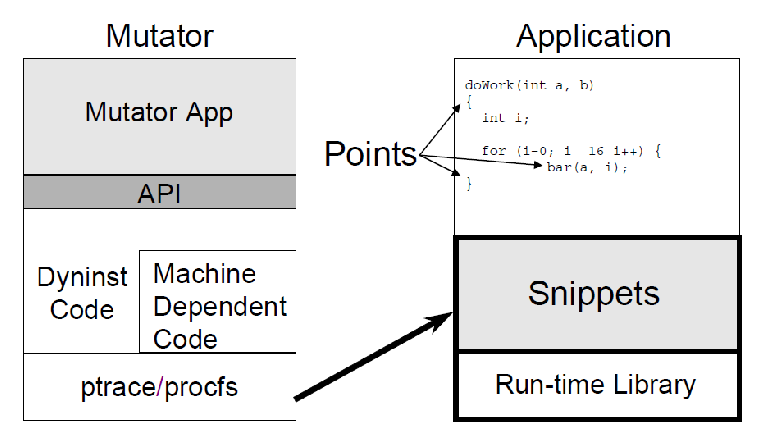
\includegraphics[width=0.6\textwidth]{dyninst.eps}
\caption{Structure of Dyninst}
\label{fig:dyninst}
\end{center}
\end{figure}

How Dyninst works is illustrated in Figure \ref{fig:dyninst}\footnote{\texttt{from Bryan's paper \cite{bib:anapi}}}. A \emph{point} is a location in a program where instrumentation can be inserted. A \emph{snippet} is a bit of binary code to be inserted into a point. The snippet is first prepared and dynamically compiled in the mutator's process space. The mutator then copies the snippet and other necessary libraries into mutatee's process space by using Linux's ptrace service. It also slightly revises the code of the \emph{point} in the mutatee to call the snippet. This way, Dyninst can insert the code into and control the execution of the mutatee.

\noindent \newline\textbf{Instrument Using Dyninst}\newline
\indent Figure \ref{fig:workflow} gives a general idea about how Dyninst works with ARUM. To do instrumentation with Dyninst, we should first integrate the Dyninst library into ARUM, then use the APIs provided by Dyninst to create a image of the application binary, prepare and insert the snippets into the specified points in the application image, then save the modified image as the new modified application binary, and finally run the new executable binary. At this point, we should have two programs running, one is the ARUM program, which is the mutator, the other is the modified application binary, which is the mutatee. The snippet in the mutatee is responsible to collect the performance data of the mutatee and send it to ARUM. After getting the data from mutatee, ARUM processes them and generates the performance report of the mutatee.

\begin{figure}
\begin{center}
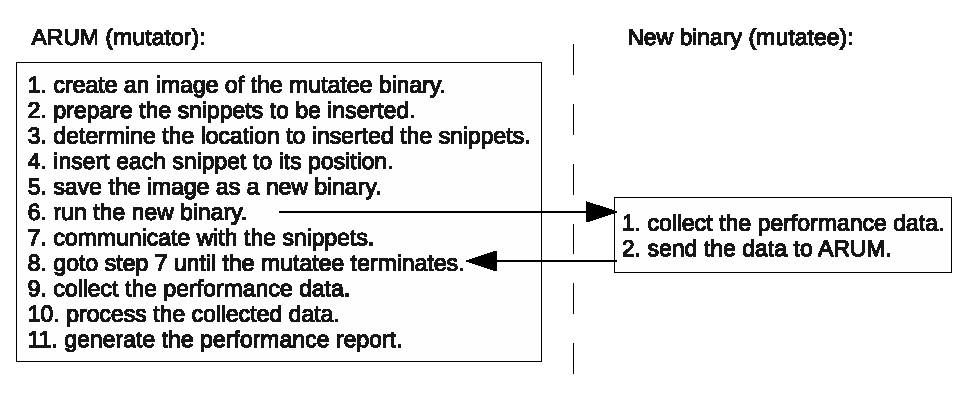
\includegraphics[width=0.9\textwidth]{workflow.eps}
\caption{Workflow of ARUM}
\label{fig:workflow}
\end{center}
\end{figure}

How the snippets are designed and where should they be inserted is the most important two question when we design our approach. The answer to these two questions depend on what performance we try to moniter. In this project, we try to profile the application program, which means we want to get how long does each function call take and how many time does each fuction is invoked. With this purpose, we designed four snippets: timestamp, isrecursive, preprocess and sendresult. The first one is used to get the timestamp of curcurrent point of execution, we use times() function in Linux. With this function, we can get the user time, system time and watch time. We insert this snippet into the beginning and the end of each function. Preprocess snippet simply collect the time at the beginning and at the end, while sendresult snippet send the result to ARUM.

There is one difficulty we encoutered. As we need to process the data at the end of the running of the function, we should have a variable to store the beginning of the time. The problem is the variable used in snippet is allocated at heap instead of at the mutatee's function stack, which means there is only one piece of memory corresponding to one function no matter how many times the function is called. So if a function is called recursively, then the inner function call will flush the result of the beginning time of the outer function call. We address this problem by introduce the isrecursive snippet, this snippet remembers if a function is called recursively or not. If yes, we don't change the value of the beginning time variable. This way, we addressed this problem by only instrumenting the top level of the function execution if the function is recursively called. All the snippets and the points where they should be inserted are illustrated in figure \ref{fig:snippet}.

\begin{figure}
\begin{center}
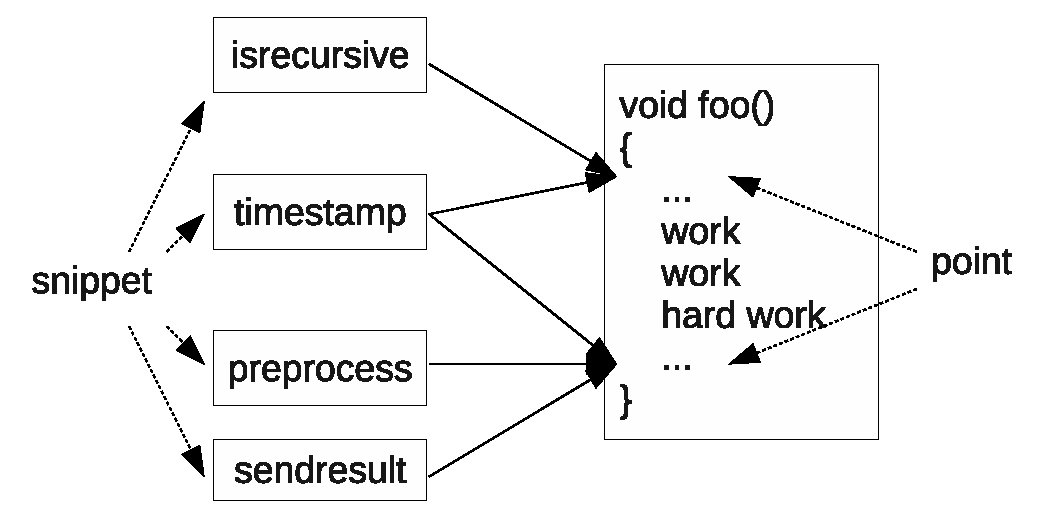
\includegraphics[width=0.6\textwidth]{snippet.eps}
\caption{Snippets and Points}
\label{fig:snippet}
\end{center}
\end{figure}

How to communicate with mutatee is another big issue. Writing the snippet code is not a trivial task, especially when we want to debug it. So it would be a good idea to make the snippet as simple as possible. We don't want to designed a complicated communication system. The method used was to simply print the result to standard output. ARUM redirected the standard output stream into a file before it launch the mutatee, and read the message from the file after the mutatee finishes.

Suppose we have a mutatee which implements four functions as shown in table \ref{tab:mutatee}. With the enhanced ARUM, we can get the profiling result looks like table \ref{tab:sampleresult}.

\begin{table}[th]
\caption{Functions in sample mutatee}
\centering
\begin{tabular}{rl}
\hline
Function & Description \\
\hline
fake & functioin never called \\
foo  & basic function \\
recursive & function call itself recursively \\
main & main function \\
\hline
\end{tabular}
\label{tab:mutatee}
\end{table}

\begin{table}[th]
\caption{Sample Result}
\centering
\begin{tabular}{rrrrrrl}
\hline
ustart & uend & sstart & send & start & end & function \\
\hline
0.00 & 0.00 & 0.00 & 0.00 & 0.00 & 0.00 & \_init \\
0.00 & 0.00 & 0.00 & 0.04 & 0.00 & 1.03 & foo \\
0.00 & 0.02 & 0.04 & 0.10 & 1.03 & 2.94 & foo \\
0.02 & 0.03 & 0.10 & 0.13 & 2.94 & 3.98 & foo \\
0.03 & 0.05 & 0.13 & 0.16 & 3.98 & 4.94 & foo \\
0.05 & 0.06 & 0.16 & 0.20 & 4.94 & 6.01 & foo \\
0.00 & 0.06 & 0.04 & 0.20 & 1.03 & 6.01 & recursive \\
0.06 & 0.08 & 0.20 & 0.22 & 6.01 & 7.76 & foo \\
0.00 & 0.08 & 0.00 & 0.22 & 0.00 & 7.76 & main \\
0.08 & 0.08 & 0.22 & 0.22 & 7.76 & 7.76 & \_fini \\
\hline
\end{tabular}
\label{tab:sampleresult}
\end{table}

For the purpose of profiling the application in binary image, we have collected enough information for further process. The collect information will look like table \ref{tab:sampleresult}. Based on this information, we can
\begin{enumerate}
\item recover the executing sequence of each function: Beginning and ending times.
\item give how many time each function runs.
\item give how long does each function instance take to run in user time, system time and watch time.
\item give the average time each function takes to run.
\item give the calling hierarchy of the functions in the application.
\end{enumerate}

The following gives the details about how we use the Dyninst APIs. By passing the application name to ARUM as an argument, ARUM can open the binary file, parse the ELF format, and create an image to represent the application executable binary. The code used to achieve this goal is shown bellow,
\begin{Verbatim}[frame=single]
handle = bpatch.openBinary(app_name);
image = handle->getImage();
\end{Verbatim}

To instrument the application, we must first decide what data want to be collected, then proper snippet should be designed carefully. This is the most chanllege and most important task. Dyninst provides a bunch of APIs to help the user to create the snippets. These APIs can support bisic arithmetic computations, general assignment, conditional assignment, loop, function call, etc... Using these APIs to write snippet code is very different from writing code using a high level language. The code shown bellow gives an example of snippet implementing increased functionality.
\begin{Verbatim}[frame=single]
count = handle->malloc(*(image->findType(``int'')));
countPlusOne = new BPatch_arithExpr(BPatch_plus, *count, BPatch_constExpr(1));
incCount = new BPatch_arithExpr(BPatch_assign, *count, *countPlusOne);
\end{Verbatim}

Having the snippet ready, we can use Dyninst to locate the position where we want to insert the snippet, and then insert our snippet there. After that, when the application runs, our snippet code will execute at certain position of the application. Of course, before we call Dyninst APIs, we should give the information about which function we are working on. The sample code to insert the above snippet is shown bellow,
\begin{Verbatim}[frame=single]
entry_point = function->findPoint(BPatch_entry);
handle->insertSnippet(*incCount,*entry_point);
\end{Verbatim}

Up to now, we can only instrument the manually specified function. With the code shown below, we can get the function list in the application and apply the above method to each of the function in the list. This way, we can automatically instrument all the functions implemented in the mutatee.
\begin{Verbatim}[frame=single]
image->findFunction(``main'', mainfuncs);
module = mainfuncs[0]->getModule();
return module->getProcedures();
\end{Verbatim}

Now, we illustrate how to build ARUM with Dyninst. After downloading Dyninst\footnote{\texttt{\url{http://www.dyninst.org/sites/default/files/downloads/dyninst/dyninst_linux_amd64_7.0.tar.gz}}}, we need install libiberty if working on linux server at PSU. The appropriate environment variables should be set according to where you put the libraries. Our settings are shown bellow,

\begin{Verbatim}[frame=single]
export LD_LIBRARY_PATH=../bprobe/lib:$LD_LIBRARY_PATH
export LD_PRELOAD=$(pwd)/../bprobe/lib/libdyninstAPI_RT.so
export DYNINSTAPI_RT_LIB=$(pwd)/../bprobe/lib/libdyninstAPI_RT.so
export DYNINST_LIBC=$(pwd)/../bprobe/lib/libc-2.13.so
\end{Verbatim}

Having set the required environment, we design our dynamic instrumentation library libbinpro.so based on Dyninst. The command used to build our library is shown bellow,

\begin{Verbatim}[frame=single]
$(CC) $(CXXFLAGS) -shared -fPIC -Wl,-rpath=./lib binpro.o -L./lib -ldyninstAPI
      -ldwarf -linstructionAPI -lsymtabAPI -lcommon -lparseAPI
      -o ./lib/libbinpro.so
\end{Verbatim}

After successfully building the library libbinpro.so, we link this library with ARUM, and make ARUM capable of dynamic instrumenation. Because the library libcommcon.so may have some unresolved function provided by libiberty.a, we need the command bellow to build ARUM,

\begin{Verbatim}[frame=single]
$(CXX) $(CXXFLAGS)-rdynamic -Wl,-rpath=../bprobe/lib $(ARCHIVE) -L../bprobe/lib
      -lbinpro -Wl,--whole-archive -liberty -Wl,--no-whole-archive
      -o $(EXE)
\end{Verbatim}

In order to solve the problem related to recursive function calls, we can just stream the timestamp to ARUM at either the beginning or the end of the function getting rid of even preprocess. If we present the beginning of the function call as \{ and the end as \}, then ARUM will get something like a stream \{\{\}\{\}\{\{\}\}\}. Problem is how to determine which end relates to which beginning. We can introduce a stack to do this easily on ARUM side.

% This should NOT be raw data or code listings.  Instead you should present the key results from your work.  Be guided by the papers you have read this quarter - in cases where it is necessary for understanding, a small section of code might be listed, separate from the text, but more commonly an algorithm might be shown.  Results are not long tables of data, rather, one or two graphs, or tables with key rows or columns highlighted or italicized.
\section{Results}
\label{sec:resultsa}

The results for the experiment is shown below.   Fig \ref{fig:orig} is result of the original version of ARUM we got from the project assignment could only output minimal information. From this point, we only get the user time and system time of the whole program. There is little value to have this information to improve the performance of the program. Fig \ref{fig:arumfact} is the result of the function list of the program output by the new version of ARUM which is extended by this project. The is the first step of our implementation. This list can give us a general idea about the size of the program. The more functions the program has, the more complex the program is. It shows the execution trace of the program. The information includes the beginning time and end time of each function of both user time and system time as well as watch time. With these information, we can figure out which function is called more and need more attention.  Fig \ref{fig:gproffact} shows a standard gprof output of the same program, which required recompiling the factorial program.   Other results with "ltrace" and "strace" would not show static function level data.

\subsection{Testing}

Test cases were developed and tested the following functionalities:
\begin{itemize}
\item Test ARUM command line options and existing functionality.
\item Test a function call.
\item Test a loop and recursive function call.
\item Test cases for multiple cascaded function calls, programs with significant execution time such as prime numbers generation, permutations of string, factorial generation with and without loop, write to file operation in loop,  a fake function to calculate time spent in a loop using difftime utility etc. 
\end{itemize}

\begin{table}[th]
\caption{Test Cases}
\centering
\begin{tabular}{ll}
\hline
Test Case & Description \\
\hline
Binary & Simple program to convert ascii values to binary \\
Loop & While loop, looping 10000000 times \\
FunctionCalls & Cascaded function calls, one of the functions in a loop, another function has loop \\
Permutation & Permutations of as string "permutation" using recursion and swap operations \\
Primes & Generate first 50000 prime numbers \\
Hello & Recursive function, a looping function, a function that is never called \\
ArumTestSpec & Program used as benchmark.
% has tests for: factorial with recursion, factorial with loop, write to file in a loop, permutations of string, prime numbers generation, a long while loop, a fake function to calculate time spent in a loop using difftime() utility \\
\end{tabular}
\label{tb:TestCases}
\end{table}

\subsection{Test Results}

% TEST RESULTS DATA
% fig 1
% TEST RESULTS FOR CODE OPTIMIZATION
% fig 2
% COMPARE ARUM PROFILING WITH GPROF PROFILING
% Arum profile information for factorial program using recursion
% fig 3
% Major Gprof profile information for factorial program using recursion
% fig 4
% fig 5

\begin{figure}
\begin{center}
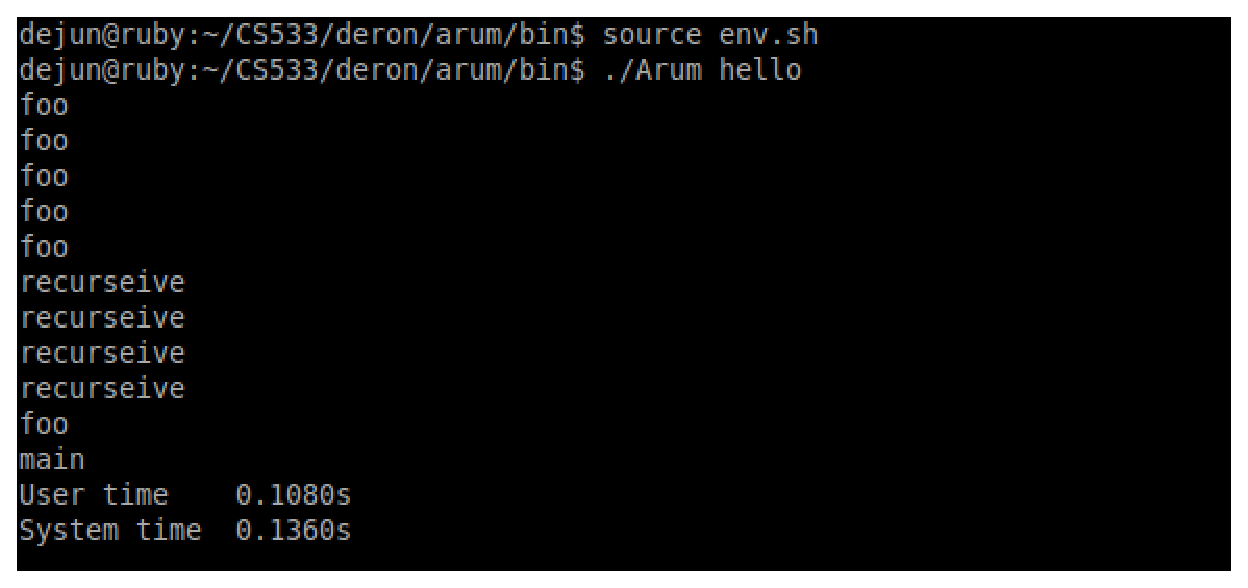
\includegraphics[width=0.8\textwidth]{orig.eps}
\caption{Output from the original ARUM}
\label{fig:orig}
\end{center}
\end{figure}

\begin{figure}
\begin{center}
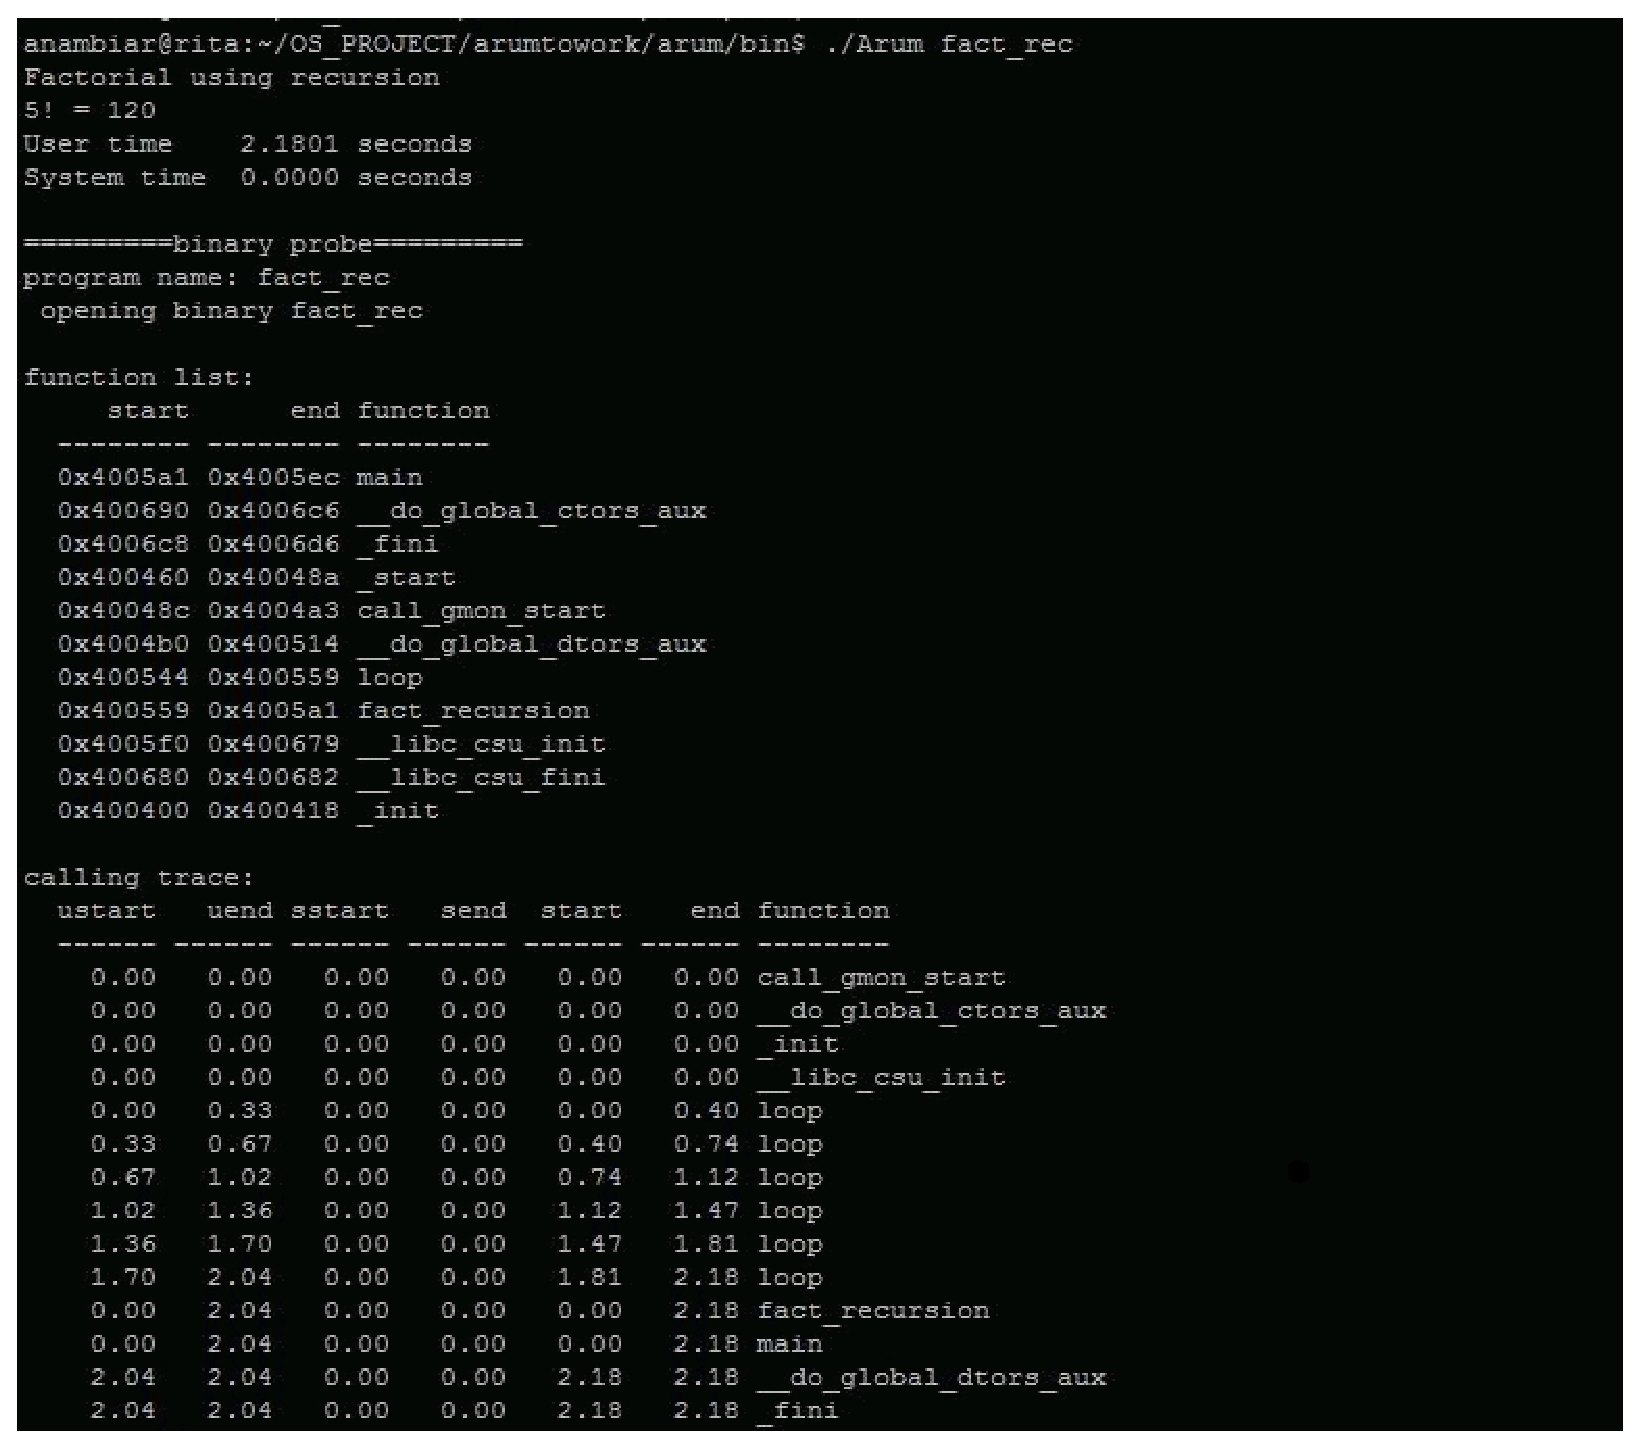
\includegraphics[width=0.8\textwidth]{arumfacttest.eps}
\caption{ARUM factorial test}
\label{fig:arumfact}
\end{center}
\end{figure}

\begin{figure}
\begin{center}
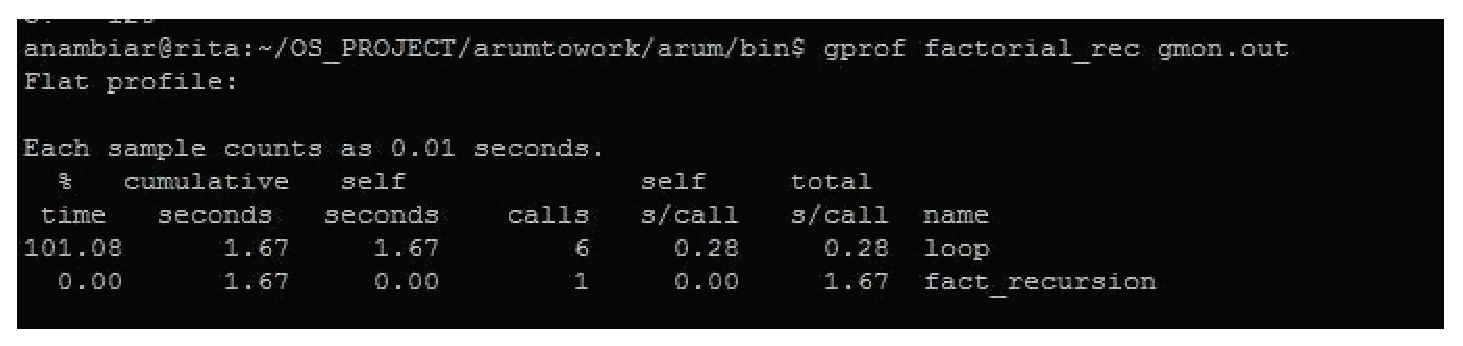
\includegraphics[width=0.8\textwidth]{gproffacttest.eps}
\caption{gprof factorial test}
\label{fig:gproffact}
\end{center}
\end{figure}

Test ARUM -r flag to report hardware counters without the HwCtr kernel module, and uses standard kernel call 'getrusage()' 

\begin{verbatim}
./Arum -r /u/anambiar/OS_PROJECT/arumtowork/arum/tests/Permutation
various permutations of string done
User time    0.0080s
System time  0.0000s
maxrss  - Max resident set size      596 Kb
minflt  - Page faults without I/O    156
majflt  - Page faults with I/O       0
inblock - File system input          48 blocks
oublock - File system output         0 blocks
nvcsw   - Voluntary context switch   8
nivcsw  - Involuntary context switch 5

\end{verbatim}

\subsection{ARUM Test Driver}

In this section we describe, ARUM Test Driver, which is a python script used to test ARUM automatically for many test cases. Test cases are given as input to the ARUM test driver in the following format. In each line, we have test name and the expected results from ARUM.\newline

{\bf Test Driver:}

\begin{verbatim}
Test Name    UserTime  SystemTime  MaxRSS  minFLT  majFLT  inBlock  outBlock

LoopTest     3.620      0.012       600     150      0        16       0

Permutation  0.004      0.004       600     158      0        48       0

Binary       0.000      0.000       600     120      0        0        0

\end{verbatim}

Our script parses each test case into input and the expected outputs. It then prepares a command to run ARUM executable along with the testname. This command is executed using a system utility function popen2.popen3(). The output is parsed in order to get UserTime, SystemTime, maxRSS, minFLT, majFLT, inBlock and outBlock parameters. These outputs are compared with the expected outputs given in the test case. If the outputs and the expected outputs are within the threshold then the test passes. In case of failures, we show the details of why the test got failed by printing the outputs and expected outputs. The following algorithm describes our python test driver for ARUM.\newline

\begin{verbatim}

Algorithm:

For each test case in test cases file

       Parse the test case for input and expected Outputs.
     
       Prepare the command which takes ARUM executable and the test name.
        (for e.g. the command will be: "./Arum -r Loop test").
       
       Run the above command using a system fumnction utility.
        (In Python it is popen2.popen3)

       Parse the standard output to get the Results.

       Compare these outputs with the expected outputs.
       
         If the outputs and the expected outputs are equal
              Print TEST is Passed
         else 
              Print TEST is Failed

              For the failed test cases:
                Print outputs and expected outputs
\end{verbatim}

{\bf Results:}\newline

The result of our test driver are shown in the following fashion. Here LoopTest and Permutation tests passed, and Binary test failed. BinaryTest failed because our Minflt and expected Minflt did not match. 

\begin{verbatim}
   LoopTest Passed

   Permutation Passed

   Binary failed
     Minflt           157
     Expected Minflt  120
\end{verbatim}
%\begin{figure}
%\begin{center}
% 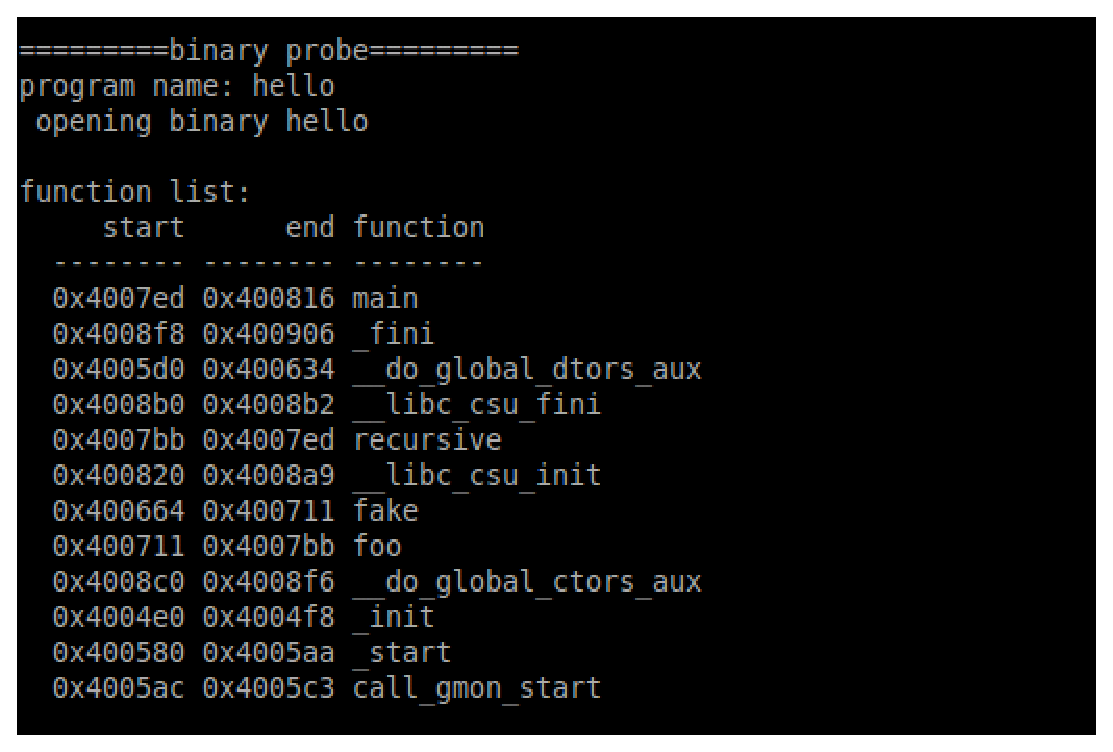
\includegraphics[width=0.7\textwidth]{list.eps}
%\caption{function list}
%\label{fig:list}
%\end{center}
%\end{figure}
%\begin{figure}
%\begin{center}
% 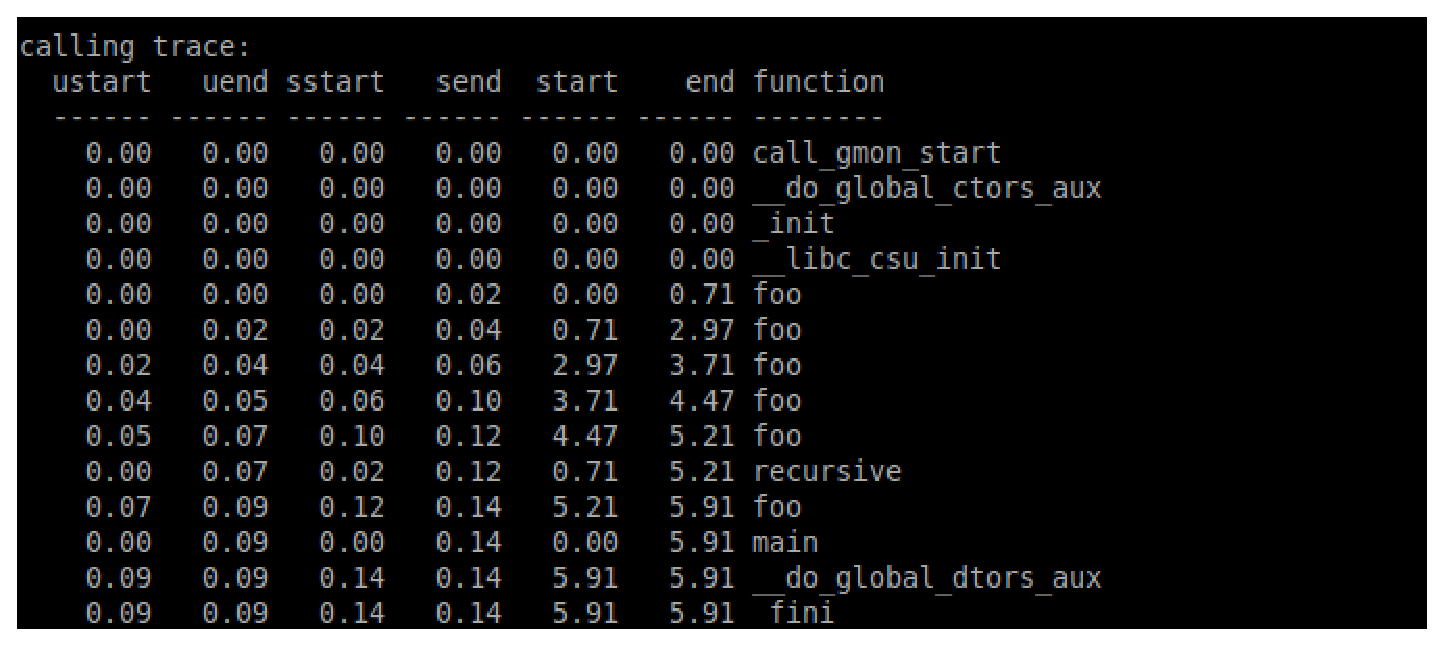
\includegraphics[width=0.9\textwidth]{trace.eps}
%\caption{execution trace}
%\label{fig:trace}
%\end{center}
%\end{figure}

% Based on what you have so far, what can you conclude?  What cool ideas did you think up but not have time to implement so far?
\section{Conclusions and Future Work}
\label{sec:conclusion}
The task of profile the application in binary mode is not trivial. We encountered the following challenges:
\begin{enumerate}
\item ARUM source code was duplicated and in several dispserse directories.  
\item Did not compile on IA32 (and other architectures).
\item HwCtr Module does not work as described in example (Don't know where the code is?)
\item Dyninst has several requirements to install and get working.
\item Can't use createProcess function. As a result, we can't inject the code into a running process. This problem is solved by rewriting the application binary before running the application.
\item Create customized structure when invoking times function to get the timestamps.
\item How to communicate with ARUM as easy as possible.
\item Handle recursive function calls.
\end{enumerate}

There is still much opportunity to improve ARUM.   One of the future goals should be to allow ARUM to run on other hardware.  The kernel module currently only supports a single architecture (Intel-15-6).  Adding the Dyninst modules to the build is extremely difficult.  Dyninst requires much work to install on various architectures and platforms.   Currently the Dyninst is compiled and commited with the project, so it will only run on single platform.  It should be added as a separate module outside of the project.  Additionally the ARUM build should link with the location of the Dyninst.
\newline
The current instrumentation works, but needs to do some formatting of the output.  The data is available, but there may be other ways to present the information to the user of the program.
\newline

% Follow a standard ACM format for your references.  You have examples in the papers you have read.
\bibliographystyle{acm}
\bibliography{reference}

%\begin{thebibliography}{9}
%\bibitem{bib:dyninst}
%\emph{http://www.dyninst.org}
%\bibitem{buck}
%Buck, B., Hollingsworth, J. \emph{An API for Runtime Code Patching}. Computer Science Department: University of Maryland. 
%\bibitem{bib:knapp}
%Knapp, R. L., Pase, D. M., Karavanic, K. L. \emph{ARUM: Application Resource Usage Monitor}.  Computer Science Department:  Portland State University.
%\end{thebibliography}

\end{document}
